\section{Introdução}

Na \ac{AGES} III, realizada no primeiro semestre de 2026, sob orientação do professor Azriel Majdenbaum, optei por participar de um projeto com proposta tecnicamente mais objetiva quando comparado ao projeto anterior, porém com elevado impacto social e grande potencial de aplicação prática. O projeto escolhido foi o \textbf{VínculoHub Portal: Plataforma de Gestão e Conexão para Organizações Sociais}, voltado à conexão entre organizações sociais e empresas interessadas em investir em iniciativas com foco social e critérios \ac{ESG}. Conforme o termo de abertura, a cliente era Kessya Carati, da Vínculo Impacta, e a turma era a 2LM4LM, com encontros às segundas e quartas-feiras, das 19h15 às 20h45. \cite{vinculotermo} A documentação do projeto complementa esta apresentação \cite{vinculohub}.

A proposta do sistema consistia em oferecer um ambiente centralizado no qual \ac{ONGs} pudessem estruturar sua presença institucional, cadastrar projetos, organizar documentos e obter maior visibilidade perante potenciais parceiros. Paralelamente, empresas poderiam localizar projetos alinhados aos seus interesses estratégicos, analisar indicadores e estabelecer vínculos institucionais de forma segura e organizada.

O termo de abertura organizava a proposta em três perfis: organizações sociais, empresas ou investidores sociais e administração da plataforma. Além de cadastros e projetos, estavam previstos acesso a editais, organização documental, relatórios e indicadores de impacto. O escopo inicial excluía sistema de pagamentos, automação de captação de recursos, aplicativo \textit{mobile} nativo, integração com sistemas governamentais externos e patrocínio social direto. Esses limites contextualizam a proposta do projeto, enquanto as seções seguintes descrevem as atividades e os resultados do desenvolvimento.

A escolha deste projeto também foi motivada pelo momento profissional em que me encontrava. Durante esta \ac{AGES}, eu já atuava no mercado como desenvolvedor de \textit{software}, o que me permitiu contribuir com maior maturidade técnica, visão prática de produto e melhor entendimento de fluxos comuns em ambientes corporativos de desenvolvimento.

Desde os primeiros encontros, percebi que o projeto possuía uma proposta diferenciada, pois unia tecnologia, organização institucional e impacto social. Além disso, havia espaço para aplicação de conhecimentos em \textit{frontend}, \textit{backend}, autenticação, modelagem de banco de dados, experiência do usuário e organização ágil de equipes.

A Figura~\ref{fig:vinculohub-equipe} apresenta a equipe do VínculoHub Portal. A atuação conjunta de alunos com diferentes experiências foi importante para organizar as frentes de produto, desenvolvimento e apoio técnico descritas neste capítulo.

\begin{figure}[!htbp]
    \centering
    \caption{Equipe do projeto VínculoHub Portal}
    \label{fig:vinculohub-equipe}
    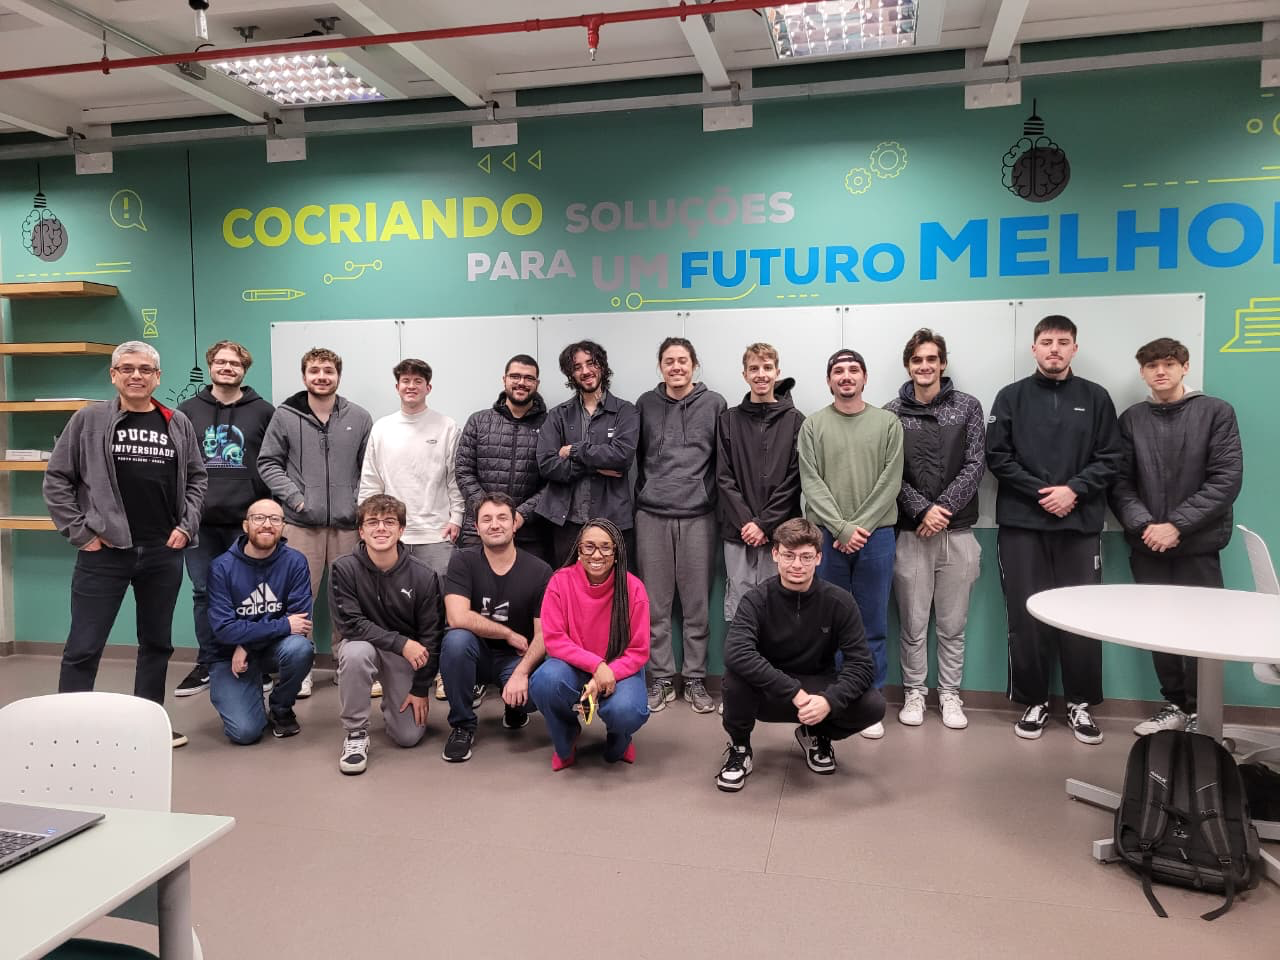
\includegraphics[width=0.9\linewidth,height=0.34\textheight,keepaspectratio]{conteudo/4 - ages III/conteudo/figures/equipe-vinculohub.png}
    \legend{Fonte: \href{https://tools.ages.pucrs.br/vinculo-hub/wiki/-/wikis/home}{wiki do projeto VínculoHub Portal}.}
\end{figure}
